%===============================================================================
% $Id: ifacconf.tex 19 2011-10-27 09:32:13Z jpuente $  
% Template for IFAC meeting papers
% Copyright (c) 2007-2008 International Federation of Automatic Control
%===============================================================================


\documentclass[a4paper]{ifacconf}
\usepackage{booktabs}
\usepackage{graphicx,amsmath,url,amssymb}      % include this line if your document contains figures
\usepackage[round]{natbib}             % required for bibliography
%===============================================================================

% ===============================================================
% Choose the language of the manuscript.
% If in English, choose 
% \def\portugues{0} 
%
% If in Portuguese or Spanish, choose
% \def\portugues{1} 
%
% Note that, if you are writing in Spanish, you need additional 
% adjusts in some parts of the text, which have been put in Portuguese only.
\def\portugues{1} 
% ===============================================================

% If the above line is commented, it is assumed manuscript in English:
\ifx\portugues\undefined
\def\portugues{0}
\fi


\if\portugues0
   \usepackage[english]{babel}
  \else
   \usepackage[spanish,brazil,english]{babel}
\fi

\usepackage[T1]{fontenc}
%\usepackage{inputenc}

\usepackage[utf8]{inputenc}
\usepackage{xcolor}
\usepackage{ae}


\if\portugues1
% =====================================================================
% =====================================================================
% If the manuscript is in Spanish, please change the texts adequatelly.
% You may also add other definitions in this part.
 \newtheorem{teorema}[thm]{{\em Teorema}}{ }
 \newtheorem{lema}[thm]{{\em Lema}}{ }
 \newtheorem{corolario}[thm]{{\em Corolário}}{ }
 \newenvironment{prova}{{\bf Prova.}}{ }
% ===============================================================
\fi

\begin{document}
	
\if\portugues1

% =====================================================================
% =====================================================================
% USE THIS PART IF THE TEXT IS IN PORTUGUES OR SPANISH
% =====================================================================
% If the manuscript is in Spanish, please change the texts adequately.
% =====================================================================
% 
\selectlanguage{brazil}
	
\begin{frontmatter}


\title{Análise de Defeitos em Células Fotovoltaicas Através da Matriz de Coocorrência de Níves de Cinza} 
% Title, preferably not more than 10 words.

\author[First]{Alan M. da Rocha} 
\author[Second]{Marcelo M. S. de Souza} 
% \author[Third]{Maria R. de Souza}

\address[First]{Universidade Federal do Ceará, Campus Mucambinho, Sobral, CE, Brasil (e-mail: eng.alanmarquesrocha@gmail.com).}
\address[Second]{Universidade Federal do Ceará, Campus Mucambinho, Sobral, CE, Brasil (e-mail: marcelo.mssouza@gmail.com)}
% \address[Third]{Instituto Federal de Educação, Ciência e Tecnologia do Ceará, Sobral, CE, Brasil (e-mail: maria.rosalia.souza06@aluno.ifce.edu.br)}


\selectlanguage{english}
\renewcommand{\abstractname}{{\bf Abstract:~}}
\begin{abstract} % Abstract of not more than 250 words.
The global demand for electricity has been gradually increasing over the 
years. To supply it, investments have been made in the generation of energy 
through renewable sources, among which photovoltaic solar energy (PV). The 
growth in the installed capacity of PV generation sources creates demands 
for sophisticated and accurate methods for detecting flaws in the cells that make up such a system. The present work proposes a method for detecting 
faults in cells of PV modules by computer vision techniques. The proposal is sensitive to the detection of shading failures, hot spots, cracks and 
micro-cracks, classifying the cells as functional or defective. The defects 
are detected by texture attributes calculated from the gray level 
co-occurrence matrix (GLCM) of the photovoltaic cell images. To verify the 
effectiveness of the classifications, cross-validation tests were performed 
on a base of photovoltaic cell images, obtained by drones, with 2624 samples divided into functional and defective classes.

\vskip 1mm% não altere esse espaçamento
\selectlanguage{brazil}
{\noindent \bf Resumo}:  A demanda global por energia elétrica vem 
aumentando gradualmente ao longo dos anos. Para supri-la, investimentos vêm 
sendo realizados na geração de energia através de fontes renováveis, dentre 
as quais a energia solar fotovoltaica (FV). O crescimento da capacidade 
instalada de fontes de geração FV criam demandas por métodos sofisticados e 
precisos para a detecção de falhas nas células que compõem tal sistema. O 
presente trabalho propõe um método para detecção de falhas em células de 
módulos FVs por técnicas de visão computacional. A proposta é sensível à 
detecção de falhas de sombreamento, pontos de calor, trincas e 
microfissuras, classificando as células como funcionais ou defeituosas. A 
detecção dos defeitos se dá por atributos de textura calculados a partir da 
matriz de coocorrência dos níveis de cinza (GLCM, do inglês Gray Level 
Co-occurrence Matrix) das imagens das células fotovoltaicas. Para verificar 
a eficácia das classificações, foram realizados testes de validação cruzada 
em uma base de imagens de células fotovoltaicas, obtidas por drones, com 
2624 amostras dividas em classes funcionais e defeituosas.
\end{abstract}

\selectlanguage{english}


\begin{keyword}
Fault Detection; Photovoltaic Cell; Computer Vision; Co-occurrence Matrix; GLCM. 

\vskip 1mm% não altere esse espaçamento
\selectlanguage{brazil}
{\noindent\it Palavras-chaves:} Detecção de Falhas; Célula Fotovoltaica; Visão Computacional; Matriz de Coocorrência; GLCM.
\end{keyword}


\selectlanguage{brazil}


\end{frontmatter}


%===============================================================================
%===============================================================================
%===============================================================================

\section{Introdução}

As mudanças climáticas produzidas pela queima de combustíveis fósseis e a dependência econômica mundial desses recursos tem estimulado a busca por alternativas renováveis de produção de energia. Neste contexto, a energia solar se destaca como uma fonte limpa, ilimitada e acessível \citep{SinghChaudhary2018}. Os sistemas de geração elétrico fotovoltaicos (FV) apresentam baixo custo de implantação, manutenção e operação \citep{Guerriero2019}. Porém, sem estratégias de proteção e detecção precoce de defeitos, esses sistemas podem sofrer falhas elétricas com custos de reparação elevados e impactantes aos consumidores. A célula fotovoltaica é o principal componente dos sistemas FVs, sendo responsável por converter a energia solar em elétrica. Para aumentar a potência produzida, essas células são associadas em série e paralelo, formando módulos, e instaladas em estruturas de painéis \citep{SinghChaudhary2018}.  

Os módulos FVs demandam inspeções periódicas para detecção e reparação preventiva de defeitos, pois estão expostos a condições ambientais, como vento, chuva, salinidade e poeira, que os degradam e comprometem a sua eficiência e confiabilidade \citep{Kim2017}. Tais inspeções podem ser realizadas indiretamente, a partir de medidas de tensões, correntes e temperaturas \citep{SanchezPacheco2014}, ou diretamente, por imagens aéreas obtidas por câmeras instaladas em Veículos Aéreos não Tripulados (VAnT). Embora o primeiro método tenha como vantagem a facilidade de obtenção das medidas, esse não permite discriminar todas as situações de falhas daquelas decorrentes de variações nas condições normais de operação \citep{Basnet2020}.  O método direto de inspeção permite a aquisição de imagens em diferentes comprimentos de onda, sendo mais comum as imagens termográficas \citep{Kim2017} e de  eletroluminescência (EL) \citep{TANG2020453}. Imagens obtidas por câmeras termográficas permitem identificar regiões defeituosas em módulos FV pelo perfil de temperatura dessas regiões, mas sem discriminar o tipo de defeito. Ademais, alguns defeitos, como micro-trincas, não produzem nenhuma alteração de temperatura e a baixa resolução das imagens termográficas degradam o desempenho do modelo de classificação de defeitos. 

A inspeção por eletroluminescência (EL) é considerada a técnica mais eficiente para avaliação da qualidade de células FV, sendo utilizada em seu processo de fabricação. Essa baseia-se no fenômeno físico de EL, que consiste na emissão de fótons na recombinação de portadores de cargas excitados sob polarização direta \citep{FRAZAO20177}. A emissão da radiação eletroluminescente é produzida estimulando as células FV com uma fonte externa de tensão. Assim, as células defeituosas apresentarão, localmente, a redução ou a perda total de emissão de radiação EL e, consequentemente, serão visualizadas como áreas escuras por câmeras que são sensíveis ao comprimento de onda da radiação emitida \citep{DJORDJEVIC2014215}. 

O presente trabalho propõe um modelo de reconhecimento de padrões, por visão computacional, para a detecção de defeitos em células fotovoltaicas a partir de imagens de EL. O modelo proposto foi validado, experimentalmente, em um conjunto de 2624 imagens aéreas de células FVs, classificadas como defeituosas (microfissuras, trincas e pontos quentes) ou não defeituosas. O modelo foi construído a partir de atributos de textura das imagens, extraídos da Matriz de Coocorrência de Níveis de Cinza (GLCM). Foram avaliados modelos com os classificadores Random Forest (RF), Support Vector Machine (SVM), Naive Bayes (NB) e K-Nearest Neighbours (kNN), sendo o classificador RF aquele que apresentou o melhor desempenho em termos de acurácia. Os resultados obtidos são competitivos em relação àqueles encontradas na literatura.  

%Os sistemas FVs frequentemente sofrem falhas elétricas relacionadas às anormalidades da configuração do sistema interno. Técnicas de identificação de defeitos em sistemas FVs são alvo de grande estudo na literatura, tendo em vista que a existência de defeitos nos módulo podem degradar diretamente a eficiência da geração de energia em grandes sistemas \citep{Li2019}. Métodos de análise e detecção de falhas através de imagens termográficas em infravermelho são propostas em \citep{BUERHOP2015}, \citep{Vergura2017} e \citep{Muttillo2020}. Outras técnicas que envolvem a análise das curvas de corrente e tensão $(I/V)$ e verificações visuais são amplamente utilizadas para a detecção de defeitos, porém dos métodos citados anteriormente, nenhum deles é capaz de verificar defeitos lineares e intrínsecos do módulo ou célula FV, gerando um diagnóstico precoce, muitas das vezes sem a possibilidade de reversão do problema. 


\section{Base de imagens}

Disponibilizada por \cite{Buerhop2018, Deitsch2018} \footnote{https://github.com/zae-bayern/elpv-dataset}, a base de imagens é composta de $2624$ amostras de imagens aéreas das células FVs de $44$ módulos. As imagens, de silício monocristalino \textit{(m-Si)} e policristalino \textit{(p-Si)}, foram obtidas por eletroluminescência e estão codificadas em níveis de cinza, corrigidas em perspectiva, padronizadas em resolução e normalizadas em dimensão, perpectiva e contraste.  

As imagens foram rotuladas como normais e defeituosas, embora as defeituosas estejam sub-divididas em classes de células com microfissuras, trincas, pontos de calor e sombreamentos. Algumas amostras estão ilustradas na Figura \ref{fig:Fig01}. 

\begin{figure}[hbt!]
\begin{center}
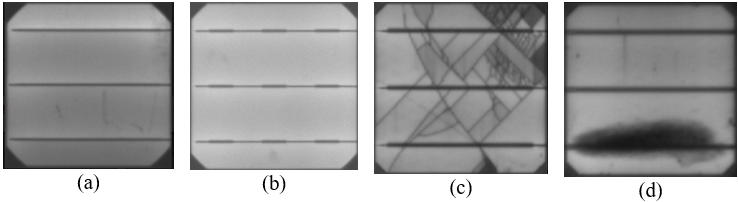
\includegraphics[width=8.4cm]{imgs/Fig01.png}    % The printed column width is 8.4 cm.
\caption{$(a)$ e $(b)$: Células de $m-Si$ em condições normais de funcionamento. $(c)$ e $(d)$: Células de $m-Si$ defeituosas com elevado nível de degradação.} 
\label{fig:Fig01}
\end{center}
\end{figure}

\section{Matriz de Coocorrência de Níveis de Cinza}

A Matriz de Coocorrência de Níveis de Cinza (GLCM) \citep{Haralick1973} descreve atributos de textura em imagens pela probabilidades de coocorrência das intensidades relativas dos pixels da imagem, segundo um critério pré-estabelecido de vizinhança. Para uma imagem com $N$ níveis de cinza, a GLCM $\mathfrak{C}$ terá dimensão $N \times N$, sendo cada elemento $\mathfrak{c}_{ij}$ de $\mathfrak{C}$ a probabilidade da coocorrência dos níveis de cinza $i$ e $j$ mediante o critério de vizinhança estabelecido.

Um elemento $\mathfrak{c_{ij}}$ de $\mathfrak{C}$ é determinado por

\begin{equation}\label{eq:01}
	\mathfrak{c_{ij}} = \{(i,j) : q \in V_p(d, \theta), i = \textbf{I}(p), j = \textbf{I}(p + q)\}, \forall{p} \in \mathfrak{D}_I 
\end{equation}   
 
, sendo $V_p(d, \theta)$ a função de vizinhança do pixel $p$, para um deslocamento $d \in \mathbb{Z}^{+}$, e uma direção $\theta \in$ \{0$^{\circ}$, 45$^{\circ}$, 90$^{\circ}$, 135$^{\circ}$\}. 

A Figura \ref{fig:Fig03} exemplifica o cálculo da GLCM de uma imagem com quatro níveis de cinza e critério de vizinhança $\theta = 0$ e $d = 1$. Na Figura \ref{fig:Fig03}(a) está em destaque todas as coocorrências das intensidades 2 e 3 na imagem, de acordo com critério de vizinhança estabelecido. A matriz GLCM da imagem está apresentada na Figura \ref{fig:Fig03}, destacando o número de coocorrências 2 e 3 encontradas na imagem.  

%A implementação do algoritmo que gera a GLCM a partir de uma imagem \textbf{I} em nível de cinza deve percorrer a matriz que representa a imagem e determinar, de acordo com as ocorrências de $(i,j)$, a quantidade de coocorrências que existem entre si, usando como base o relacionamento espacial. 

%preenchimento da matriz, utilizam-se técnicas de extração de atributos de  textura, visando encontrar as características mais relevantes. Neste trabalho  utilizou-se 04 das 14 medidas estatísticas propostas por Haralick, para descrever as 
%texturas \citep{Haralick1973}. Muitos desses atributos são correlacionados entre si e acrescentam pouca  capacidade de discriminação. Um subconjunto desses atributos, especificado como segue,  é o mais frequentemente utilizado em aplicações práticas.

A partir da GLCM pode-se calcular os seguintes atributos de textura: 

\begin{figure}[hbt!]
\begin{center}
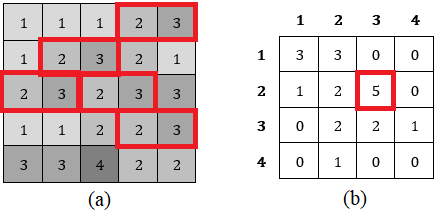
\includegraphics[width=8.4cm]{imgs/Fig03.png}    % The printed column width is 8.4 cm.
\caption{(a) Uma imagem contendo $N_g = 4$ níveis de cinza. (b) Exemplo de GLCM para a vizinhança de um pixel à direita $(\mathfrak{C}$ para $d = 1$, $\theta =$ 0$^{\circ}$).} 
\label{fig:Fig03}
\end{center}
\end{figure}

\begin{itemize}
    \item Contraste $(Con)$: Realiza a medição da intensidade de um pixel e verifica sua similaridade com o pixel vizinho. Segundo \citep{Ramalho2013}, valores concentrados na diagonal mostram que não existe contraste na imagem. Se os maiores pesos estiverem fora da diagonal, então existirá um aumento significativo do contraste. A Equação (\ref{eq:02}) mostra a definição do descritor de contraste, em que $k \geq 1$ define o quão rápido a medida deve variar com a distância
    da diagonal. Para $k = 1$ e $l = 1$ essa medida se torna uma medida de dissimilaridade de primeira ordem.

    \begin{equation}\label{eq:02}
	    Con = \sum_{i,j = 0}^{N_g - 1} |i-j|^k (\mathfrak{c_{ij}})^l\
    \end{equation}   
 
    \item Homogeneidade $(Hom$ ou $Mdi)$: Mede o quanto a distribuição dos elementos da GLCM está próxima da diagonal. Esta medida também é chamada de momento de diferença inverso $Mdi$ e pode ser calculada conforme a Equação (\ref{eq:03}).
    
    \begin{equation}\label{eq:03}
	    Hom = \sum_{i,j = 0}^{N_g - 1} \frac{\mathfrak{c_{ij}}}{1 + |i-j|}\
    \end{equation}
    
    \item Entropia $(Ent)$: É possível medir a aleatoriedade dos níveis de cinza de \textbf{I} através de $Ent$ utilizando a Equação (\ref{eq:04}). 
    
     \begin{equation}\label{eq:04}
	    Ent = \sum_{i,j = 0}^{N_g - 1}{\mathfrak{c_{ij}}}\ln({\mathfrak{c_{ij}}})\
    \end{equation}
    
    \item Segundo momento angular $(ASM$): O $ASM$ mede a homogeneidade de \textbf{I} através da correlação de pares $P(i,j)$ de quase toda a área da imagem, independente das distâncias de $(i,j)$. A $ASM$ pode ser calculada conforme a Equação (\ref{eq:05}).
    
     \begin{equation}\label{eq:05}
	    ASM = \sum_{i,j = 0}^{N_g - 1} P(i,j)^2\
    \end{equation}
    
     \end{itemize}	


O processo de transformar uma GLCM em uma aproximação de uma tabela de probabilidades é chamado de normalização. Logicamente que, para se obter a GLCM, a imagem deve primeiramente ser segmentada e representada em níveis de cinza, conforme exemplificado na Figura \ref{fig:Fig03}. O tamanho da matriz irá depender da quantidade de níveis de cinza. Ela possui um número de linhas $(M_i)$ e um número de colunas $(M_j)$ iguais a quantidade de níveis de cinza \citep{HARALICK1992}. 

\section{Extração de atributos}

Os atributos de textura da GLCM, empregados na identificação de defeitos das células FVs, foram calculados através das funções \textit{greycomatrix()} e \textit{greycoprops()} da biblioteca de processamento de imagem \textit{scikit-image} \citep{van_der_Walt_2014}. A primeira calcula  GLCMs de uma imagem, tendo os parâmetros descritos na Tabela \ref{Tab:00}. Cada GLCM calculada por \textit{greycomatrix()} corresponde a um par cartesiano $(d,\theta)$. Já a segunda calcula as estatísticas das GLCMs, tendo como parâmetros as GLCMs calculadas por \textit{greycomatrix()} e a lista das propriedades estatísticas desejadas, dentre aquelas definidas nas Equações \ref{eq:02} a \ref{eq:05}.


\begin{table*}[h]	
	\centering
	\caption{Parâmetros da função \textit{greycomatrix()} para o cálculo da GLCM}\label{Tab:00}
		\begin{tabular}{cp{0.5\textwidth}}
		   \hline \textbf{Parâmetro} & \textbf{Descrição} \\ \hline
			 \textit{Image} & Imagem em níveis de cinza\\
			 \textit{Distances} & Lista dos deslocamentos ($d$) nas quais as vizinhanças serão consideradas para o cálculo das coocorrências. \\
          \textit{Angles} & Lista de ângulos ($\theta$), em radianos, das direções nas quais as vizinhanças serão consideradas no cálculo das coocorrências.\\
          \textit{levels} &Número de níveis de cinza (256 para 8 bits).\\
			 \textit{symmetric} & Variável lógica que indica se as coocorrências serão simétricas ($(i, j)$ = $(j, i)$).\\
			 \textit{normed} & Variável lógica que indica  se a GLCM será normalizada como probabilidade.\\
			 \hline
		\end{tabular}
\end{table*}


As três estruturas horizontais observadas na Figura~\ref{fig:Fig02} (a) são denominadas de busbars (BB). Essas consistem em filamentos metálicos para a condução de corrente elétrica através das células FVs. A partir dessas estruturas, estabelecemos quatro regiões de interesse (ROI), como ilustrado na Figura~\ref{fig:Fig02} (b), e calculamos GLCMs, variando os parâmetros $(\textit{d},\theta)$, em cada uma delas. Obtivemos então, para cada ROI, um conjunto de GLCMs (Figura \ref{fig:Fig04}), sendo as propriedadas estatísticas de cada GLCM, calculadas e concatenadas, par compor um único vetor de atributos de cada ROI. Por fim, os vetores de atributos das quatro ROI são concatenados para comporem o descritor da célula FV empregado nos experimentos de classificação (Figura \ref{fig:Fig05}).  


\begin{figure}[hbt!]
\begin{center}
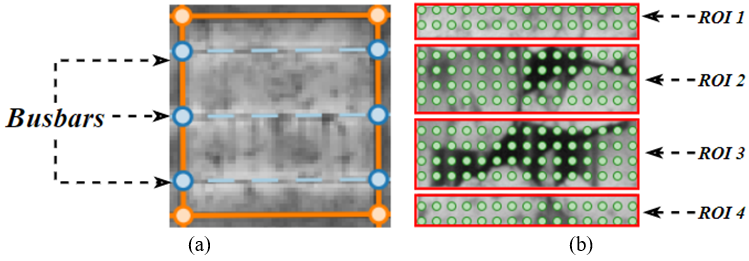
\includegraphics[width=8.4cm]{imgs/Fig02.png}    % The printed column width is 8.4 cm.
\caption{$(a)$ \textit{Busbars} das células FVs. (b) Regiões de interesse da célula FV.} 
\label{fig:Fig02}
\end{center}
\end{figure}



\begin{figure*}[hbt!]
\begin{center}
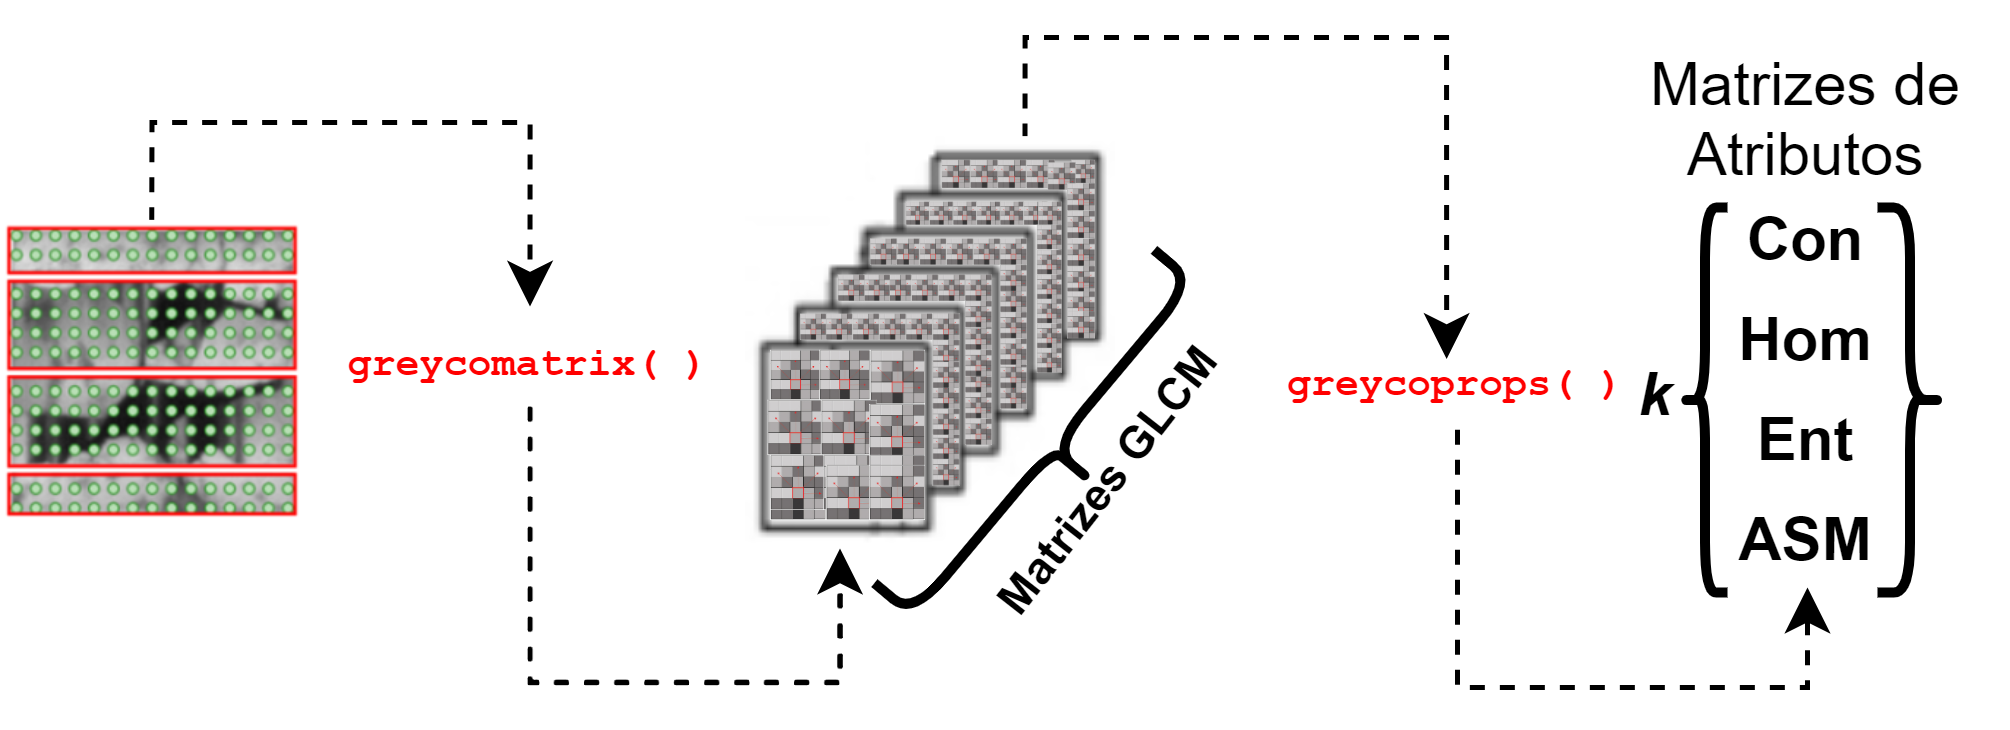
\includegraphics[width=14cm]{imgs/Fig04.png}    % The printed column width is 8.4 cm.
\caption{Obtenção das GLCMs e atributos das imagens da célula FV.} 
\label{fig:Fig04}
\end{center}
\end{figure*}

\section{Experimentos de classificação}

A avaliação experimental do modelo é representada pelo fluxo ilustrado na Figura \ref{fig:Fig05}, aonde todos os atributos obtidos de cada imagem, através das GLCMs, são concatenados e normalizados para média zero e variância unitária. Selecionam-se então os melhores atributos, pelo critério estatístico de análise de variância (ANOVA), para por fim validar o modelo por validação cruzada \textit{Kfold ($K = 4$)}.

Após calcularmos as matrizes de atributos equivalentes, concatenou-se os resultados obtidos formando-se a matriz $\mathfrak{M_c}$ com todos os atributos de textura da imagem. Por fim, utilizou-se a função \textit{SelectKBest} para escolher os melhores atributos de $\mathfrak{M_c}$ utilizadas nas validações cruzadas de teste e treino por meio do método \textit{k-fold} \citep{7544814}, tendo como passo seguinte realizar as classificações das imagens por meio dos classificadores: RF, SVM, NB e KNN.

\begin{figure*}[hbt!]
\begin{center}
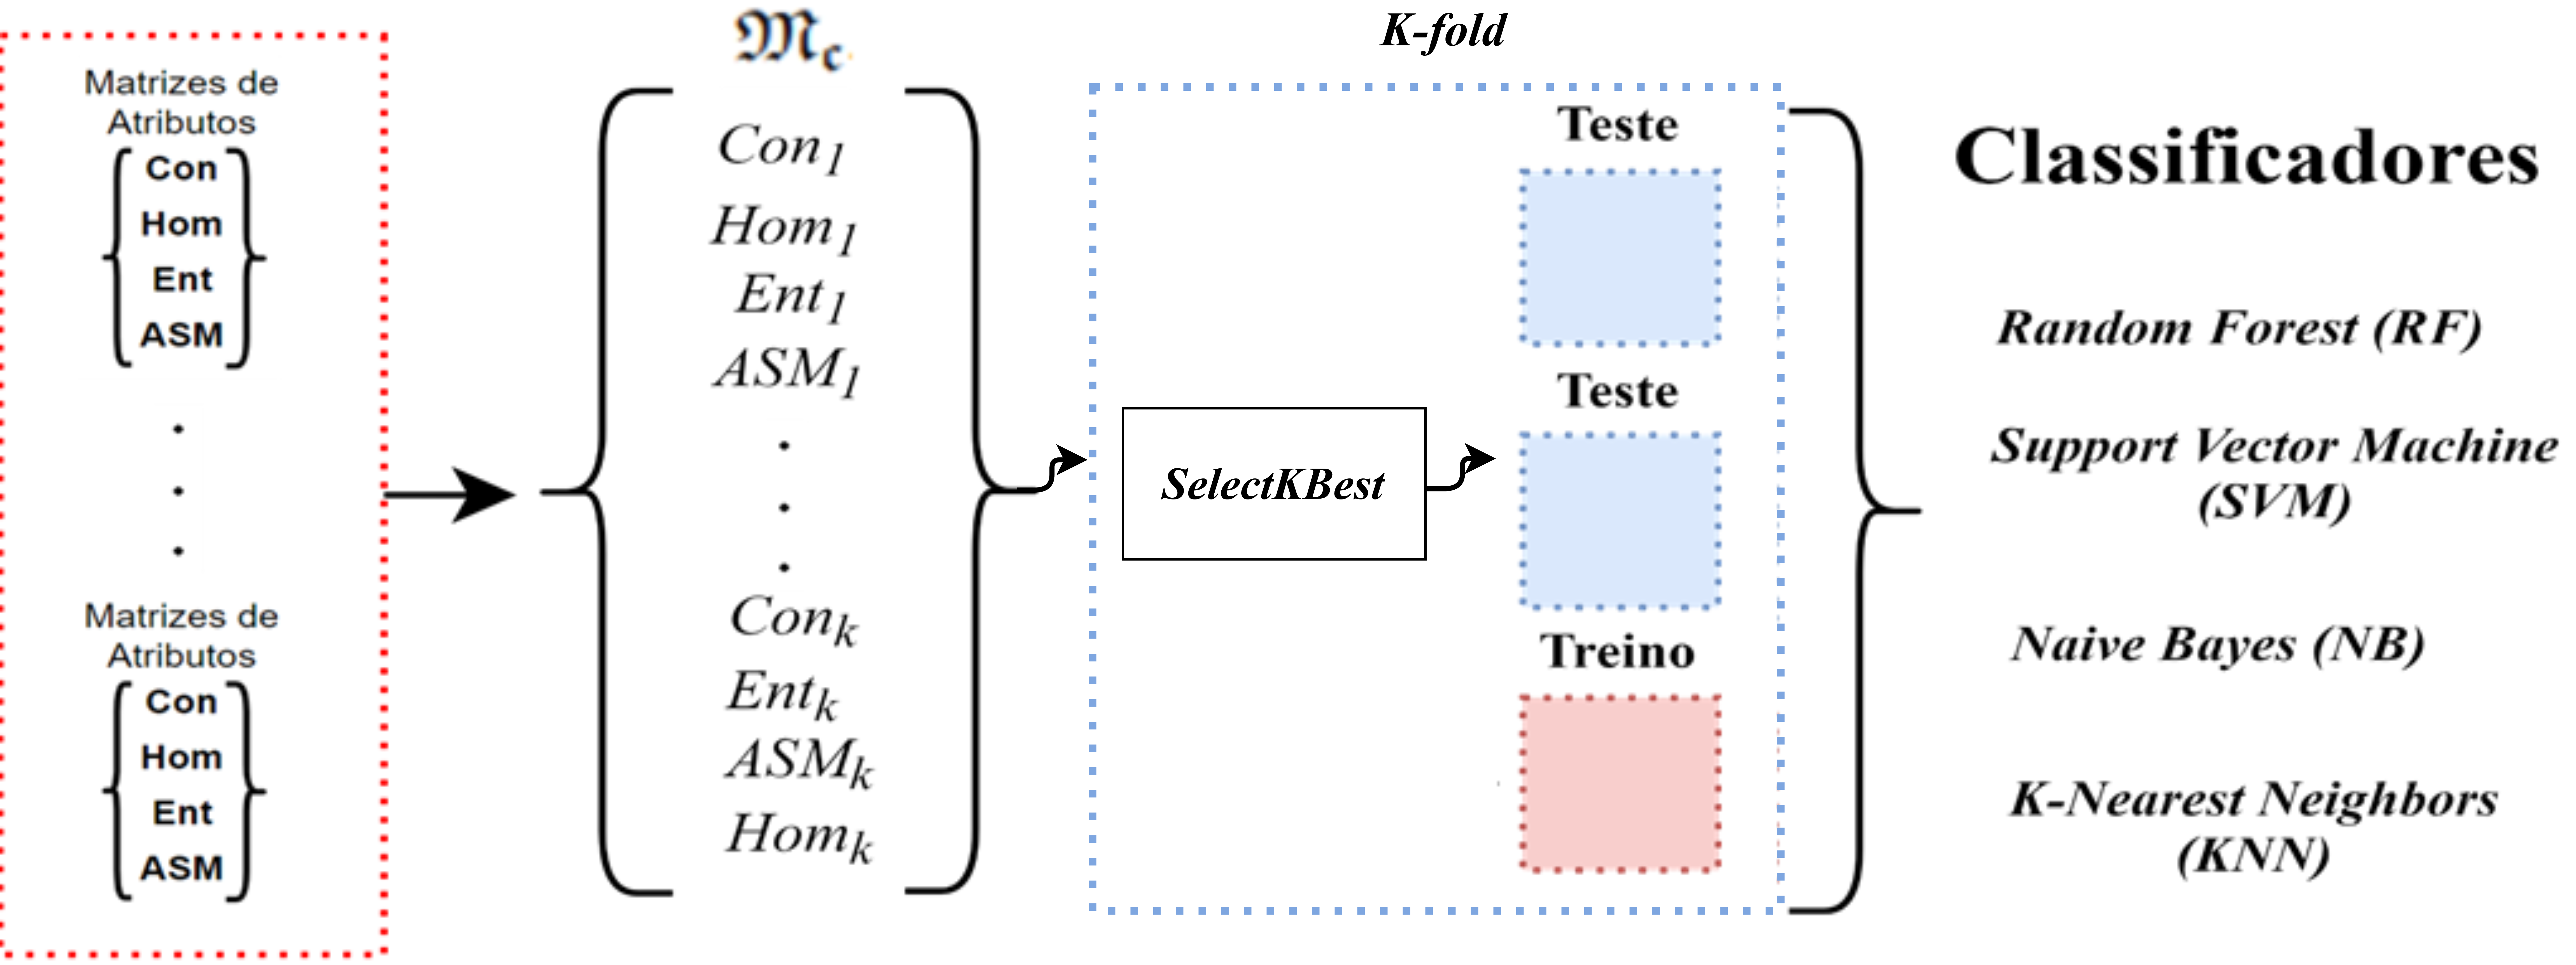
\includegraphics[width=14cm]{imgs/Fig05.png}    % The printed column width is 8.4 cm.
\caption{Cálculo das propriedades de textura e validação cruzada pelo método \textit{k-fold.}} 
\label{fig:Fig05}
\end{center}
\end{figure*}


\subsection{Classificadores}

Para verificar a eficácia da divisão das classes de imagens em defeituosas e funcionais, utilizamos quatro classificadores implementados na biblioteca em Python \textit{scikit-learn}:

%seguindo o processo definido pela Figura \ref{fig:Fig06}. 

%\begin{figure}[hbt!]
%\begin{center}
%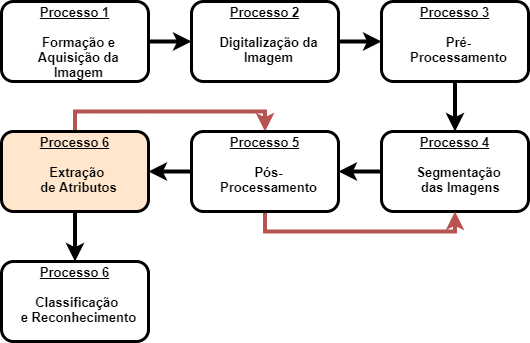
\includegraphics[width=6.4cm]{imgs/Fig06.png}    % The printed column width is 8.4 cm.
%\caption{Diagrama para o processamento das imagens enfatizando a extração de atributos.} 
%\label{fig:Fig06}
%\end{center}
%\end{figure}

%Assim, implementando os seguintes classificadores:

\textbf{SVM:} A SVM é um tipo de aprendizado de máquina (ML) que discrimina um conjunto de amostras de teste dividindo-o em dois grupos, em outras palavras é um classificador binário em sua formulação original \citep{Oliveira2011}.

\textbf{NB:} O classificador NB aprende a partir dos dados de treinamento a probabilidade condicional de cada atributo dado o valor da classe, fornecendo uma abordagem simples, com semântica limpa, para representar, usar e aprender conhecimento probabilístico \citep{SantosLazeraWanke2014}.

\textbf{KNN:}  O algoritmo de KNN realiza o armazenamento e classificação de uma classe de interesse através da comparação entre as similaridades da classe de interesse por meio dos dados de teste \citep{Buani2009}. 

\textbf{RF:} É um algoritmo de aprendizado supervisionado não paramétrico usado para classificação e regressão. O objetivo é criar um modelo que preveja o valor de uma variável de destino, aprendendo regras de decisão simples inferidas dos recursos de dados. Uma árvore pode ser vista como uma aproximação constante por partes.

\section{Métricas de avaliação}
O modelo foi avaliado através das seguintes métricas de classificação:

\begin{itemize}
    \item \textbf{Matriz de confusão (MC): }A MC tem por finalidade, relacionar os resultados corretos de uma classificação com os resultados previstos pelo modelo de reconhecimento de padrões, faciliando a visualização do número de classificações corretas e do número de classificaç~es preditas para cada classe de um determinado conjunto de testes.
    
    \begin{table}[hb]
      \begin{center}
        \caption{Matriz de confusão para classificação binária}\label{tb:01}
          \begin{tabular}{cccc}
      & \textbf{Classe Positiva} & \textbf{Classe Negativa} \\\hline
      Positiva Real & VP & FN \\
      Negativa Real & FP & VN \\ \hline
\end{tabular}
\end{center}
\end{table}

Onde, VP é o número de predições positivas, VN é o número de predições negativas, FP é a falsa predição positiva e FN é a falsa predição negativa.   

 \item \textbf{Acurácia (ACC): } A acurácia avalia o quão efetivo um classificador é, por meio da probabilidade do algorimo de realizar predições corretas e pode ser calculada conforme a Equação (\ref{eq:06}).
 
 \begin{equation}\label{eq:06}
	ACC = \frac{|VN|+|VP|}{|FN|+|FP|+|VN|+|VP|}.
\end{equation} 

 \item \textbf{Sensibilidade, Precisão e F-Score: } Algumas medidas são utilizadas especificamente em classificações binárias, como por exemplo as medidas de sensibilidade $(S_s)$, precisão $(P)$ e \textit{F-Score} e podem ser calculadas através das Equações (\ref{eq:07}), (\ref{eq:08}) e (\ref{eq:09}), respectivamente.
 
 \begin{equation}\label{eq:07}
	S_s = \frac{|VP|}{|VP|+|FN|}
\end{equation} 

\begin{equation}\label{eq:08}
	P = \frac{|VP|}{|VP| + |FP|}
\end{equation}

\begin{equation}\label{eq:09}
	F-Score = \frac{(2 \times P \times S_s)}{(P + S_s)}
\end{equation}
 
\end{itemize}

\section{Resultados e Discussão}

%\subsection{Desempenho em Classificação}

%Os resultados a seguir serão apresentados sob a perspectiva das medidas de avaliação de desempenho $ACC$, $S_s$, $P$ e $F-Score$. 

A Tabela \ref{tab:02} apresenta os resultados do  primeiro experimento de validação cruzada, aonde calcularam-se a acurácia dos classificadores de acordo com o número dos melhores atributos selecionados da $\mathfrak{M_c}$. Em negrito, destacam-se os melhores resultados, sendo o classificador RF aquele que obteve o melhor desempenho, com acurácias de 90\% para 410 atributos, seguido pela SVM, que obteve 87\% de acurácia para 110 atributos, e o NB, com 85\% de acurácia para 710 atributos. Por fim, o KNN obteve acurácia de 84\% para 210 atributos.

\begin{table}[h]	
	\centering
	\caption{Resultado da Acurácia (ACC) dos classificadores com os 1110 atributos de $\mathfrak{M_c}$.}\label{tab:02}
		\begin{tabular}{ccccc}
			    \hline \textbf{Atributos} & \textbf{RF} & \textbf{SVM} & \textbf{NB} & \textbf{KNN}\\ \hline
			 10 & 0,85$\pm$0,06 & 0,81$\pm$0,07 & 0,81$\pm$0,07 & 0,83$\pm$0,07 \\
			 110 & 0,89$\pm$0,05 & \textbf{0,87}$\pm$0,05 & 0,82$\pm$0,05 & 0,81$\pm$0,06 \\
			 210 & 0,89$\pm$0,05 & 0,85$\pm$0,05 & 0,83$\pm$0,07 & \textbf{0,84}$\pm$0,05 \\
			 310 & 0,89$\pm$0,05 & 0,85$\pm$0,04 & 0,81$\pm$0,07 & \textbf{0,84}$\pm$0,08 \\
			 410 & \textbf{0,90}$\pm$0,03 & 0,85$\pm$0,06 & 0,82$\pm$0,06 & 0,82$\pm$0,06 \\
			 510 & 0,89$\pm$0,04 & 0,85$\pm$0,03 & 0,82$\pm$0,05 & 0,82$\pm$0,07 \\
			 610 & 0,88$\pm$0,04 & 0,84$\pm$0,05 & 0,83$\pm$0,03 & 0,80$\pm$0,06 \\
			 710 & 0,87$\pm$0,05 & 0,84$\pm$0,04 & \textbf{0,85}$\pm$0,04 & 0,83$\pm$0,06 \\
			 810 & 0,88$\pm$0,02 & 0,85$\pm$0,04 & 0,83$\pm$0,02 & 0,82$\pm$0,04 \\
			 910 & 0,89$\pm$0,03 & \textbf{0,86}$\pm$0,02 & 0,83$\pm$0,03 & 0,83$\pm$0,06 \\
			 1110 & \textbf{0,90}$\pm$0,03 & 0,85$\pm$0,04 & \textbf{0,84}$\pm$0,05 & 0,83$\pm$0,04 \\
			\hline
		\end{tabular}
\end{table}

As métricas de  Sensibilidade $(S_s)$, Precisão $(P)$ e $F-Score$ estão dispostas nas Tabelas \ref{tab:03}, \ref{tab:04} e \ref{tab:05}, respectivamente, nos quais foram utilizados os 880 melhores atributos da matriz $\mathfrak{M_c}$ nos experimentos.

\begin{table}[h]	
	\centering
	\caption{Resultado dos classificadores por meio da Sensibilidade $(S_s)$ com os 880 atributos de $\mathfrak{M_c}$.}\label{tab:03}	
		\begin{tabular}{ccccc}\hline
			    \textbf{Atributos} & \textbf{RF} & \textbf{SVM} & \textbf{NB} & \textbf{KNN}\\ \hline
			 80 & 0,85$\pm$0,04 & 0,83$\pm$0,05 & 0,84$\pm$0,07 & 0,83$\pm$0,05 \\
			180 & 0,84$\pm$0,08 & 0,84$\pm$0,06 & 0,85$\pm$0,07 & \textbf{0,86}$\pm$0,06 \\
			280 & 0,85$\pm$0,07 & 0,83$\pm$0,05 & \textbf{0,86}$\pm$0,07 & \textbf{0,86}$\pm$0,07 \\
			380 & 0,86$\pm$0,08 & \textbf{0,85}$\pm$0,07 & 0,87$\pm$0,05 & 0,86$\pm$0,08 \\
			480 & 0,85$\pm$0,09 & \textbf{0,85}$\pm$0,08 & 0,85$\pm$0,07 & 0,84$\pm$0,05 \\
			580 & 0,86$\pm$0,05 & 0,82$\pm$0,09 & 0,84$\pm$0,13 & 0,86$\pm$0,06 \\
			680 & \textbf{0,88}$\pm$0,06 & 0,83$\pm$0,07 & 0,84$\pm$0,07 & 0,85$\pm$0,07 \\
			780 & 0,87$\pm$0,04 & 0,84$\pm$0,08 & \textbf{0,86}$\pm$0,07 & 0,85$\pm$0,07 \\
			880 & \textbf{0,90}$\pm$0,05 & 0,85$\pm$0,05 & 0,84$\pm$0,02 & 0,84$\pm$0,06 \\
			\hline
		\end{tabular}
\end{table}

Na Tabela \ref{tab:03} são apresentadas as medidas de $S_s$ dos quatro classificadores, a métrica obtida por eles, estima a probabilidade das células com defeito e funcionais serem classificadas de acordo com a sua respectiva classe, isto quer dizer por exemplo que, para um conjunto de cem células FVs com defeito, com $S_s=93\%$, mostra que o classificador realizou a predição corretamente de 93 das 100 imagens. Neste caso,  Verifica-se mais uma vez que o classificador RF obteve o melhor resultado: 90\% para 880 atributos, seguido dos classificadores NB e KNN com 86\% para 180, 280 e 780 atributos em suas melhores classificações. O algoritmo SVM sofreu uma pequena redução de sua métrica, quando comparado com os resultados das Tabelas \ref{tab:02} e \ref{tab:03}. 

\begin{table}[h]	
	\centering
	\caption{Resultado dos classificadores por meio da Precisão $(P)$ com os 880 atributos de $\mathfrak{M_c}$.}\label{tab:04}
		\begin{tabular}{ccccc} \hline
			    \textbf{Atributos} & \textbf{RF} & \textbf{SVM} & \textbf{NB} & \textbf{KNN}\\ \hline
			 80 & 0,92$\pm$0,06 & \textbf{0,92}$\pm$0,08 & 0,91$\pm$0,04 & \textbf{0,93}$\pm$0,05 \\
			180 & 0,91$\pm$0,06 & 0,89$\pm$0,08 & 0,91$\pm$0,06 & 0,93$\pm$0,07 \\
			280 & 0,90$\pm$0,06 & 0,89$\pm$0,06 & 0,91$\pm$0,05 & 0,93$\pm$0,05 \\
			380 & 0,93$\pm$0,06 & 0,89$\pm$0,04 & 0,92$\pm$0,07 & \textbf{0,94}$\pm$0,05 \\
			480 & 0,91$\pm$0,03 & \textbf{0,90}$\pm$0,05 & 0,93$\pm$0,06 & 0,93$\pm$0,06 \\
			580 & \textbf{0,93}$\pm$0,03 & 0,88$\pm$0,07 & \textbf{0,94}$\pm$0,04 & 0,91$\pm$0,06 \\
			680 & 0,91$\pm$0,05 & 0,88$\pm$0,05 & 0,94$\pm$0,05 & 0,92$\pm$0,05 \\
			780 & 0,92$\pm$0,04 & 0,88$\pm$0,06 & 0,94$\pm$0,06 & 0,92$\pm$0,04 \\
			880 & \textbf{0,94}$\pm$0,05 & 0,86$\pm$0,05 & \textbf{0,94}$\pm$0,04 & 0,92$\pm$0,05 \\
			\hline
		\end{tabular}
\end{table}

A Tabela \ref{tab:04} apresenta as medidas de $(P)$. Observa-se claramente que a probabilidade da predição positiva estar correta foi bem avaliada por todos os classificadores, sendo o NB mais bem avaliado com uma precisão de 94\% e desvio padrão de $\pm$ 4\% com 580 e 880 atributos, seguindo do RF com 94\% e desvio padrão de $\pm$ 5\% para 880 atributos, empatado com o classificador KNN com a mesma precisão, mas com 380 atributos. Por fim, o SVM obteve a menor precisão, mas ainda assim considerada ótima com 90\% para 480 atributos. Os resultados da Tabela \ref{tab:04} demonstram que tando as células consideradas defeituosas, quando as funcionais foram classificadas de forma eficaz. Deve-se salientar que não houve mudança nos parâmetros dos respectivos algoritmos e que os resultados obtidos podem ser verificados por meio da MC.

\begin{table}[h]	
	\centering
	\caption{Resultado dos classificadores por meio da métrica \textit{F-Score} com os 880 atributos de $\mathfrak{M_c}$.}\label{tab:05}

		\begin{tabular}{ccccc}
	            \hline
			    \textbf{Atributos} & \textbf{RF} & \textbf{SVM} & \textbf{NB} & \textbf{KNN}\\
			\hline
			 80 & 0,86$\pm$0,05 & \textbf{0,88}$\pm$0,06 & \textbf{0,83}$\pm$0,05 & \textbf{0,83}$\pm$0,07 \\
			180 & 0,87$\pm$0,04 & \textbf{0,87}$\pm$0,04 & \textbf{0,81}$\pm$0,08 & 0,82$\pm$0,04 \\
			280 & 0,88$\pm$0,05 & 0,85$\pm$0,04 & 0,80$\pm$0,06 & 0,81$\pm$0,05 \\
			380 & 0,88$\pm$0,05 & 0,87$\pm$0,05 & 0,80$\pm$0,05 & 0,82$\pm$0,06 \\
			480 & \textbf{0,89}$\pm$0,05 & 0,85$\pm$0,06 & 0,80$\pm$0,07 & 0,82$\pm$0,08 \\
			580 & 0,88$\pm$0,04 & 0,86$\pm$0,05 & 0,80$\pm$0,07 & 0,81$\pm$0,04 \\
			680 & \textbf{0,90}$\pm$0,05 & 0,85$\pm$0,05 & 0,80$\pm$0,07 & 0,82$\pm$0,05 \\
			780 & 0,88$\pm$0,04 & 0,86$\pm$0,05 & 0,80$\pm$0,07 & \textbf{0,83}$\pm$0,05 \\
			880 & 0,89$\pm$0,05 & 0,86$\pm$0,04 & 0,80$\pm$0,06 & 0,82$\pm$0,06 \\
			\hline
		\end{tabular}
\end{table}

Os resultados apresentados na Tabela \ref{tab:05} representam a combinação das métricas de precisão e sensibilidade, de forma balanceada, calculada através da Equação (\ref{eq:09}). Os resultados obtidos foram semelhantes às métricas de $S_s$ e $ACC$.

No experimento para calcularmos a última métrica, o classificador RF se destacou dentre os outros, tendo como melhor resultado uma métrica de 90\%, seguida da SVM com 88\%, KNN com 83\% nos dois melhores casos e o NB com 83\% no primeiro melhor caso e 81\% no segundo.  Comparando-se os resultados dos classificadores NB e KNN, observamos que os mesmos realizam predições de formas semelhantes, isso só foi possível devido as mudanças de parâmetros do KNN. Uma comparação das métricas obtidas através dos experimentos realizados com os classificadores é essencial para podermos finalmente encontrar o melhor classificador dentre os quatro utilizados. Fazendo inicialmente a média da métrica \textit{F-Score} podemos então verificar qual classificador obteve a menor taxa de erro em suas classificações. O resultado calculado pode ser observado na Tabela \ref{tab:06}.

\begin{table}[h]	
	\centering 
	\caption{Média \textit{F-Score} dos classificadores.}\label{tab:06}	
		\begin{tabular}{ccccc}\hline
			    \textbf{$F-Score$} & \textbf{RF} & \textbf{SVM} & \textbf{NB} & \textbf{KNN}\\
			\hline
			 \textbf{Média} & \textbf{0,88$\pm$0,05} & 0,86$\pm$0,06 & 0,80$\pm$0,06 & 0,82$\pm$0,05 \\
			\hline
		\end{tabular}
\end{table}

O classificador RF se consolidou como o melhor dentre os quatro utilizados neste trabalho, chegando a uma média final de 88\% e desvio padrão de 5\%. Sua melhor classificação
ocorreu através da métrica de precisão com 92\% e desvio padrão de 5\%. Um dos motivos para que o RF seja tão preciso em classificações binárias é porque o mesmo combina centenas ou milhares de árvores de decisão (DTs), treina cada uma em um conjunto ligeiramente diferente de observações, dividindo nós em cada árvore considerando um número limitado de atributos. As previsões finais do RF são feitas pela média das previsões de cada árvore individual

%\subsection{Desempenho dos Classificadores pela Matriz de Confusão (MC)}

As predições ilustradas na Figura \ref{fig:07} $(a)$ apresentam os valores exatos da classificação realizada na primeira validação. O RF classificou 94 imagens de células FVs funcionais (VP) de forma correta, tendo uma classificação incorreta (FP) de 15 imagens. Já para a classificação de células defeituosas (VN), o RF classificou 111 imagens de forma efetiva, contra 16 imagens que apresentaram problemas, mas foram classificadas como funcionais.

Na segunda validação o RF classificou 101 imagens de células FVs funcionais de forma correta, tendo realizado a classificação de 22 imagens que são caracterizadas como defeituosas, de forma funcional. Em relação as imagens defeituosas, o RF classificou 104 imagens de forma efetiva, enquanto que 9 imagens de células que não são consideradas defeituosas, foram classificadas com defeito.

\begin{figure}[hbt!]
\begin{center}
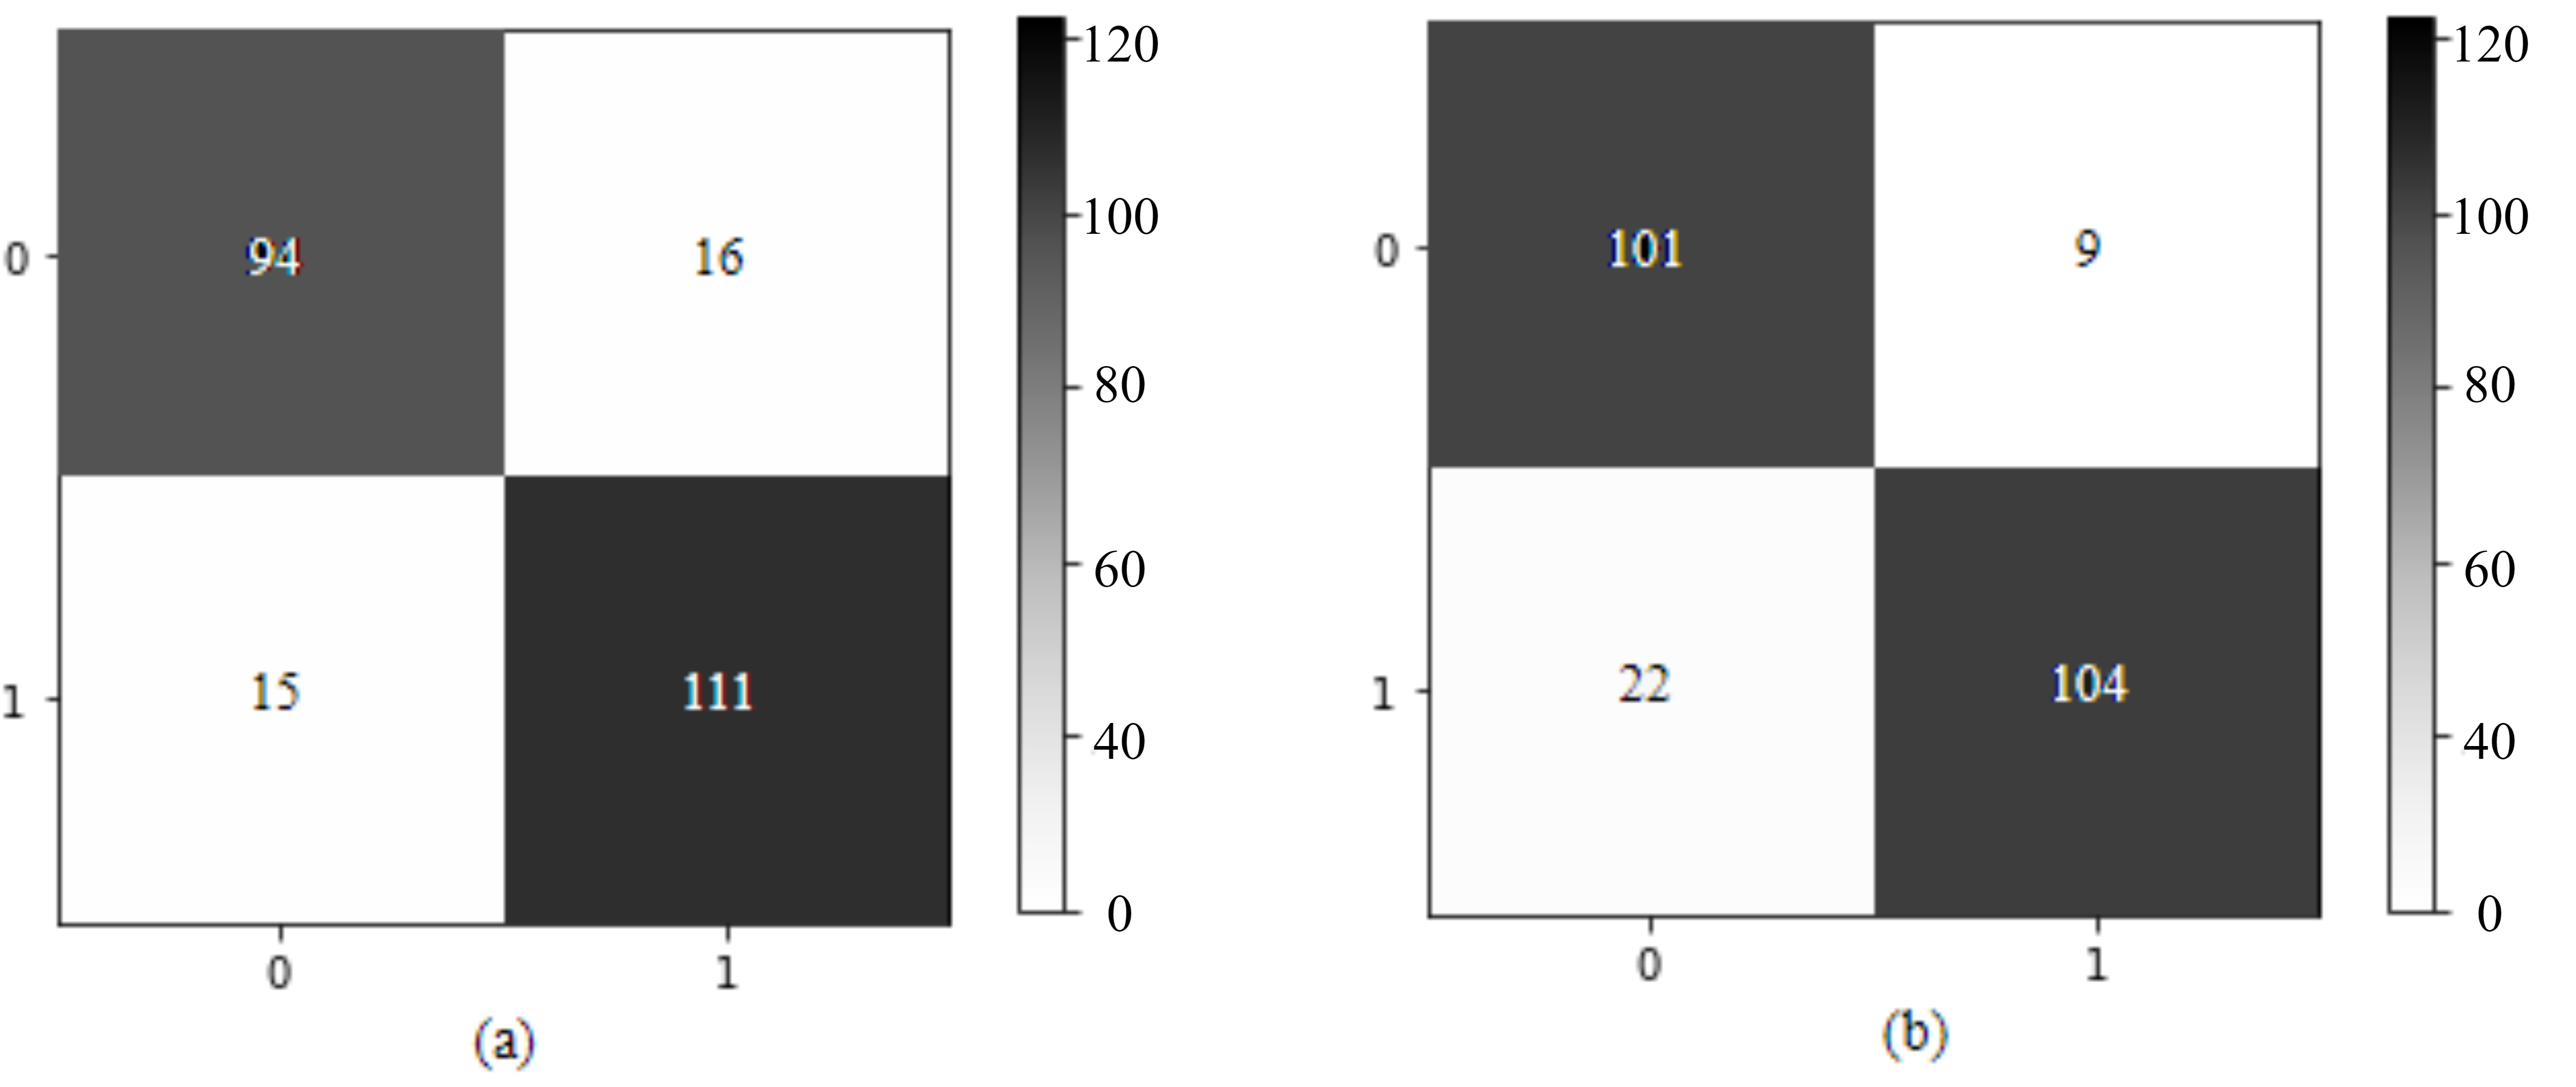
\includegraphics[width=8.4cm]{imgs/Fig07.png}    % The printed column width is 8.4 cm.
\caption{(a) Matriz de confusão para o classificador SVM na 1ª validação. (b) Matriz de confusão do classificador SVM na 2ª validação.} 
\label{fig:07}
\end{center}
\end{figure}

A Figura \ref{fig:08} $(a)$ ilustra a imagem de uma célula FV que foi classificada como funcional na primeira validação, mas que possui microfissuras difíceis de serem classificadas, mas que podem diminuir a eficiência da célula. A Figura \ref{fig:08} $(b)$ ilustra uma célula FV que deveria ter sido classificada como defeituosa na primeira validação, mas foi classificada como funcional. Já a Figura \ref{fig:08} $(c)$ ilustra a imagem de uma célula FV que foi classificada como funcional na segunda validação, mas que possui uma microfissura quase imperceptível. Por fim, a Figura \ref{fig:08} $(d)$ ilustra uma célula FV que deveria ter sido classificada como defeituosa na segunda validação, mas que foi classificada como funcional.

\begin{figure}[hbt!]
\begin{center}
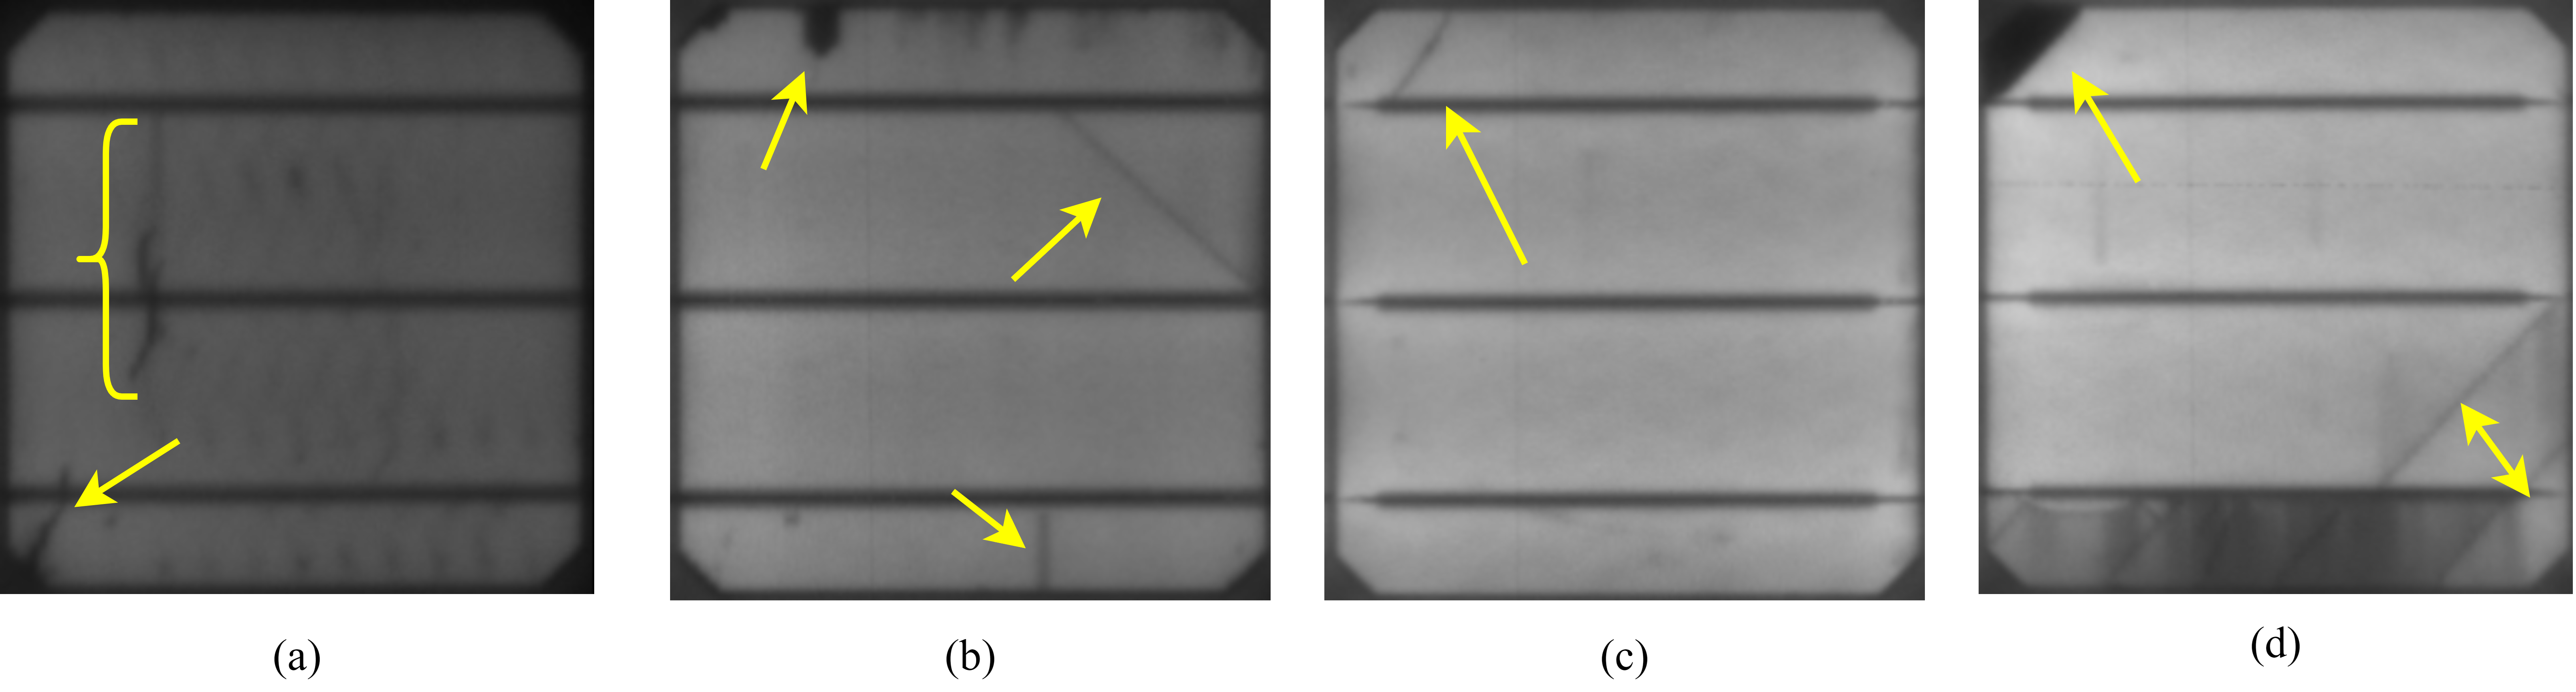
\includegraphics[width=8.4cm]{imgs/Fig08.png}    % The printed column width is 8.4 cm.
\caption{(a) FP da 1ª validação com o  Random Forest. (b) FN da 1ª validação com o Random Forest. (c) FP da 2ª validação com o Random Forest. (d) FN da 2ª validação com o Random Forest.} 
\label{fig:08}
\end{center}
\end{figure}

Os níveis de defeito das células FVs presentes no banco de dados foram rotulados através de estimativas que poderiam variar de 0 a 1, onde 0 seria uma célula completamente funcional e 1 seria completamente defeituosa. Essas métricas foram estabelecidas nos trabalhos de \citep{Deitsch2018, Buerhop2018, Deitsch2019}. A Figura \ref{fig:09} apresenta algumas imagens de células FVs que foram classificadas corretamente através dos classificadores RF e SVM. Observa-se nas Figuras \ref{fig:09} $(a)$ e $(c)$ que o níveis de degradação em certas células são bastante visíveis (trincas, pontos quentes e microfissuras), já em outros casos, a classificação por meio visual seriam difíceis de serem encontradas. 

\begin{figure}[hbt!]
\begin{center}
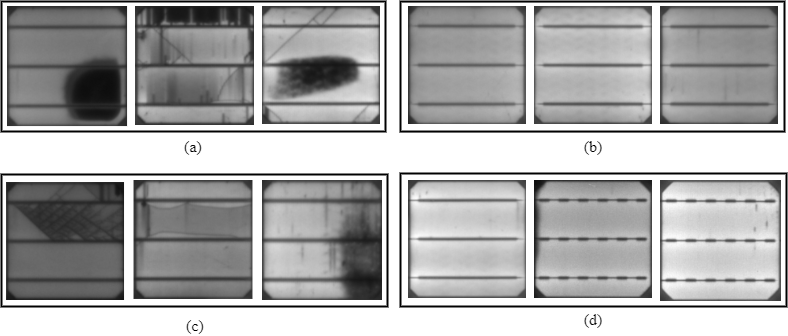
\includegraphics[width=8.4cm]{imgs/Fig09.png}    % The printed column width is 8.4 cm.
\caption{(a) Células FVs com defeito classificadas corretamente pelo RF. (b) Células FVs funcionais classificadas corretamente pelo RF (c) Células FVs com defeito classificadas corretamente pela SVM. (d) Células FVs funcionais classificadas corretamente pela SVM.} 
\label{fig:09}
\end{center}
\end{figure}

\subsection{Comparações com Trabalhos Presentes na Literatura}

Nesta seção, comparamos os resultados de nossa metodologia com aqueles encontrados na literatura, propondo verificar a eficácia do método proposto. 
A Tabela \ref{tab:07} apresenta os resultados obtidos por trabalhos que utilizaram a mesma base de imagens de células FVs utilizadas para realizar a classificação em defeituosas e funcionais.


\begin{table}[h]	
	\centering 
	\caption{Comparações com trabalhos relacionados.}\label{tab:07}	
		\begin{tabular}{llr}
			\cmidrule(r){1-3}
                \textbf{Autores} & \textbf{Algoritmo Proposto} & \textbf{Acurácia}\\ \midrule
                \midrule
                \citep{Deitsch2019} & SVM & 84,44\% \\
                & CNN & 88,42\% \\ 
                \hline
                \citep{Shin2020} & SVM & 64,00\% \\
                & CNN & 64,00\% \\
                & RF & 63,00\% \\
                & LR & 63,00\% \\
                & SGD & 62,00\% \\
                \hline
                \citep{Akram2019} & CNN & 93,02\% \\
                 &  &  \\
                \hline
                Elaborado pelo Autor & RF & 90,00\% \\
                & SVM & 87,00\% \\
                & NB & 85,00\% \\
                & KNN & 85,00\% \\
                \bottomrule
		\end{tabular}
\end{table}



No trabalho de \citep{Deitsch2019}, foram utilizadas 1968 imagens do banco de dados de \citep{Buerhop2018} e que foi tomado como referência neste trabalho. O método proposto realiza duas abordagens para a detecção automática dos defeitos das células FVs. Na primeira, se fez o uso de uma SVM, obtendo uma acurácia de 82.44\%. A segunda abordagem utilizou uma Rede Neural Convolucional (CNN), obtendo uma acurácia final de 88.42\%. 

Em \citep{Shin2020}, foram utilizadas as 2624 imagens do banco de dados de \cite{Buerhop2018}, implementando os métodos de classificação SVM, RF, \textit{Logistic Regression (LR)}, \textit{Stochastic Gradient Descent (SGD)} e KNN. Os resultados obtidos por meio da acurácia de cada classificador foram de 64\% para a SVM e RF, 63\% para os classificadores \textit{LR} e \textit{SGD} e 62\% para o KNN. Comparando os parâmetros dos classificadores RF, SVM e KNN, no trabalho de \citep{Shin2020}, foram utilizadas 100 árvores e 5 amostras mínimas para realizar a divisão de um nó interno para cada interação. O \textit{kernel} utilizado na SVM foi o \textit{Radial Basis Function (RBF)} e o valor de $k$ do classificador KNN foi de 5. 

No trabalho de \citep{Akram2019}, também foi utilizado o banco de dados de \citep{Buerhop2018}. O trabalho utilizou para o reconhecimento de defeitos em imagens EL, obtendo resultados de até 93,02\% no conjunto de dados. Os experimentos foram realizados através da arquitetura VGG-19 com 8 \textit{layers}, VGG-16 com 7 \textit{layers} e VGG-11 com 6 \textit{layers}.

Em todos os trabalhos citados acima os resultados obtidos foram próximos das médias dos classificadores apresentados neste trabalho, evidenciando o RF com uma média de acurácia de 88\% e a SVM com uma acurácia de 86\%, competindo diretamente com os trabalhos de \cite{Deitsch2019, Akram2019}. 


\section{Conclusões}
Neste trabalho, foi proposto a detecção de falhas em células de módulos fotovoltaicos de silício monocristalino e policristalino através da análise dos atributos de uma GLCM. As imagens em níveis de cinza foram dividas em vetores de atributos, nos quais
foram calculados pelas estatísticas de contraste, homogeneidade, entropia e segundo momento
angula, propostas por \citep{Haralick1973}. A matriz resultante com todos os atributos foi
dividida por meio da validação cruzada para que fossem escolhidos os melhores atributos por
meio da classe SelectKBest. Os classificadores foram implementados com parâmetros específicos,
nos quais foram escolhidos de forma empírica. Em termos de acurácia, o classificador RF obteve o melhor resultado (90\%), seguido da SVM com 87\%. Como resultado final, utilizando a média da métrica $F-Score$, o classificador RF consolidou-se como o melhor proposto neste trabalho, apresentando um resultado de 88\%. Por
meio das matrizes de confusão do RF, verificou-se que o mesmo classificou corretamente 94
imagens de células FVs funcionais (verdadeiro positivo) de forma correta, tendo uma classificação
incorreta (falso positivo) de 15 imagens. Já para a classificação de células defeituosas (verdadeiro
negativo), o RF classificou 111 imagens de forma efetiva, contra 16 imagens que apresentaram
problemas, mas foram classificadas como funcionais. 
da SVM com 87\%. 

\bibliography{ifacconf}             % bib file to produce the bibliography
                                                     % with bibtex (preferred)


\end{document}
